\section{Podsumowanie i testy stacji}

Testy stacji stanowiły testy części radiowej i konstrukcyjnej. W ramach grantu kupiono balon na misję balonową, aby wraz z układem z poprzedniego grantu przetestować łącze radiowe w praktycznych warunkach.

\subsection{Część konstrukcyjna}

Test stanowił sprawdzenie współpracy z oprogramowaniem Orbitron do ustawiania pozycji. W tym celu kazaliśmy stacji wodzić za stacją ISS będącą najszybciej poruszającym się obiektem na bliskiej orbicie. Stacja nie miała problemu aby nadążyć za instrukcjami, więc test zakończył się sukcesem.



Poniżej zdjęcia z przebiegu testów, na których widać orientację anteny i zrzut ekran z programu Orbitron w danej chwili.

\begin{figure}[h]
	\centering
		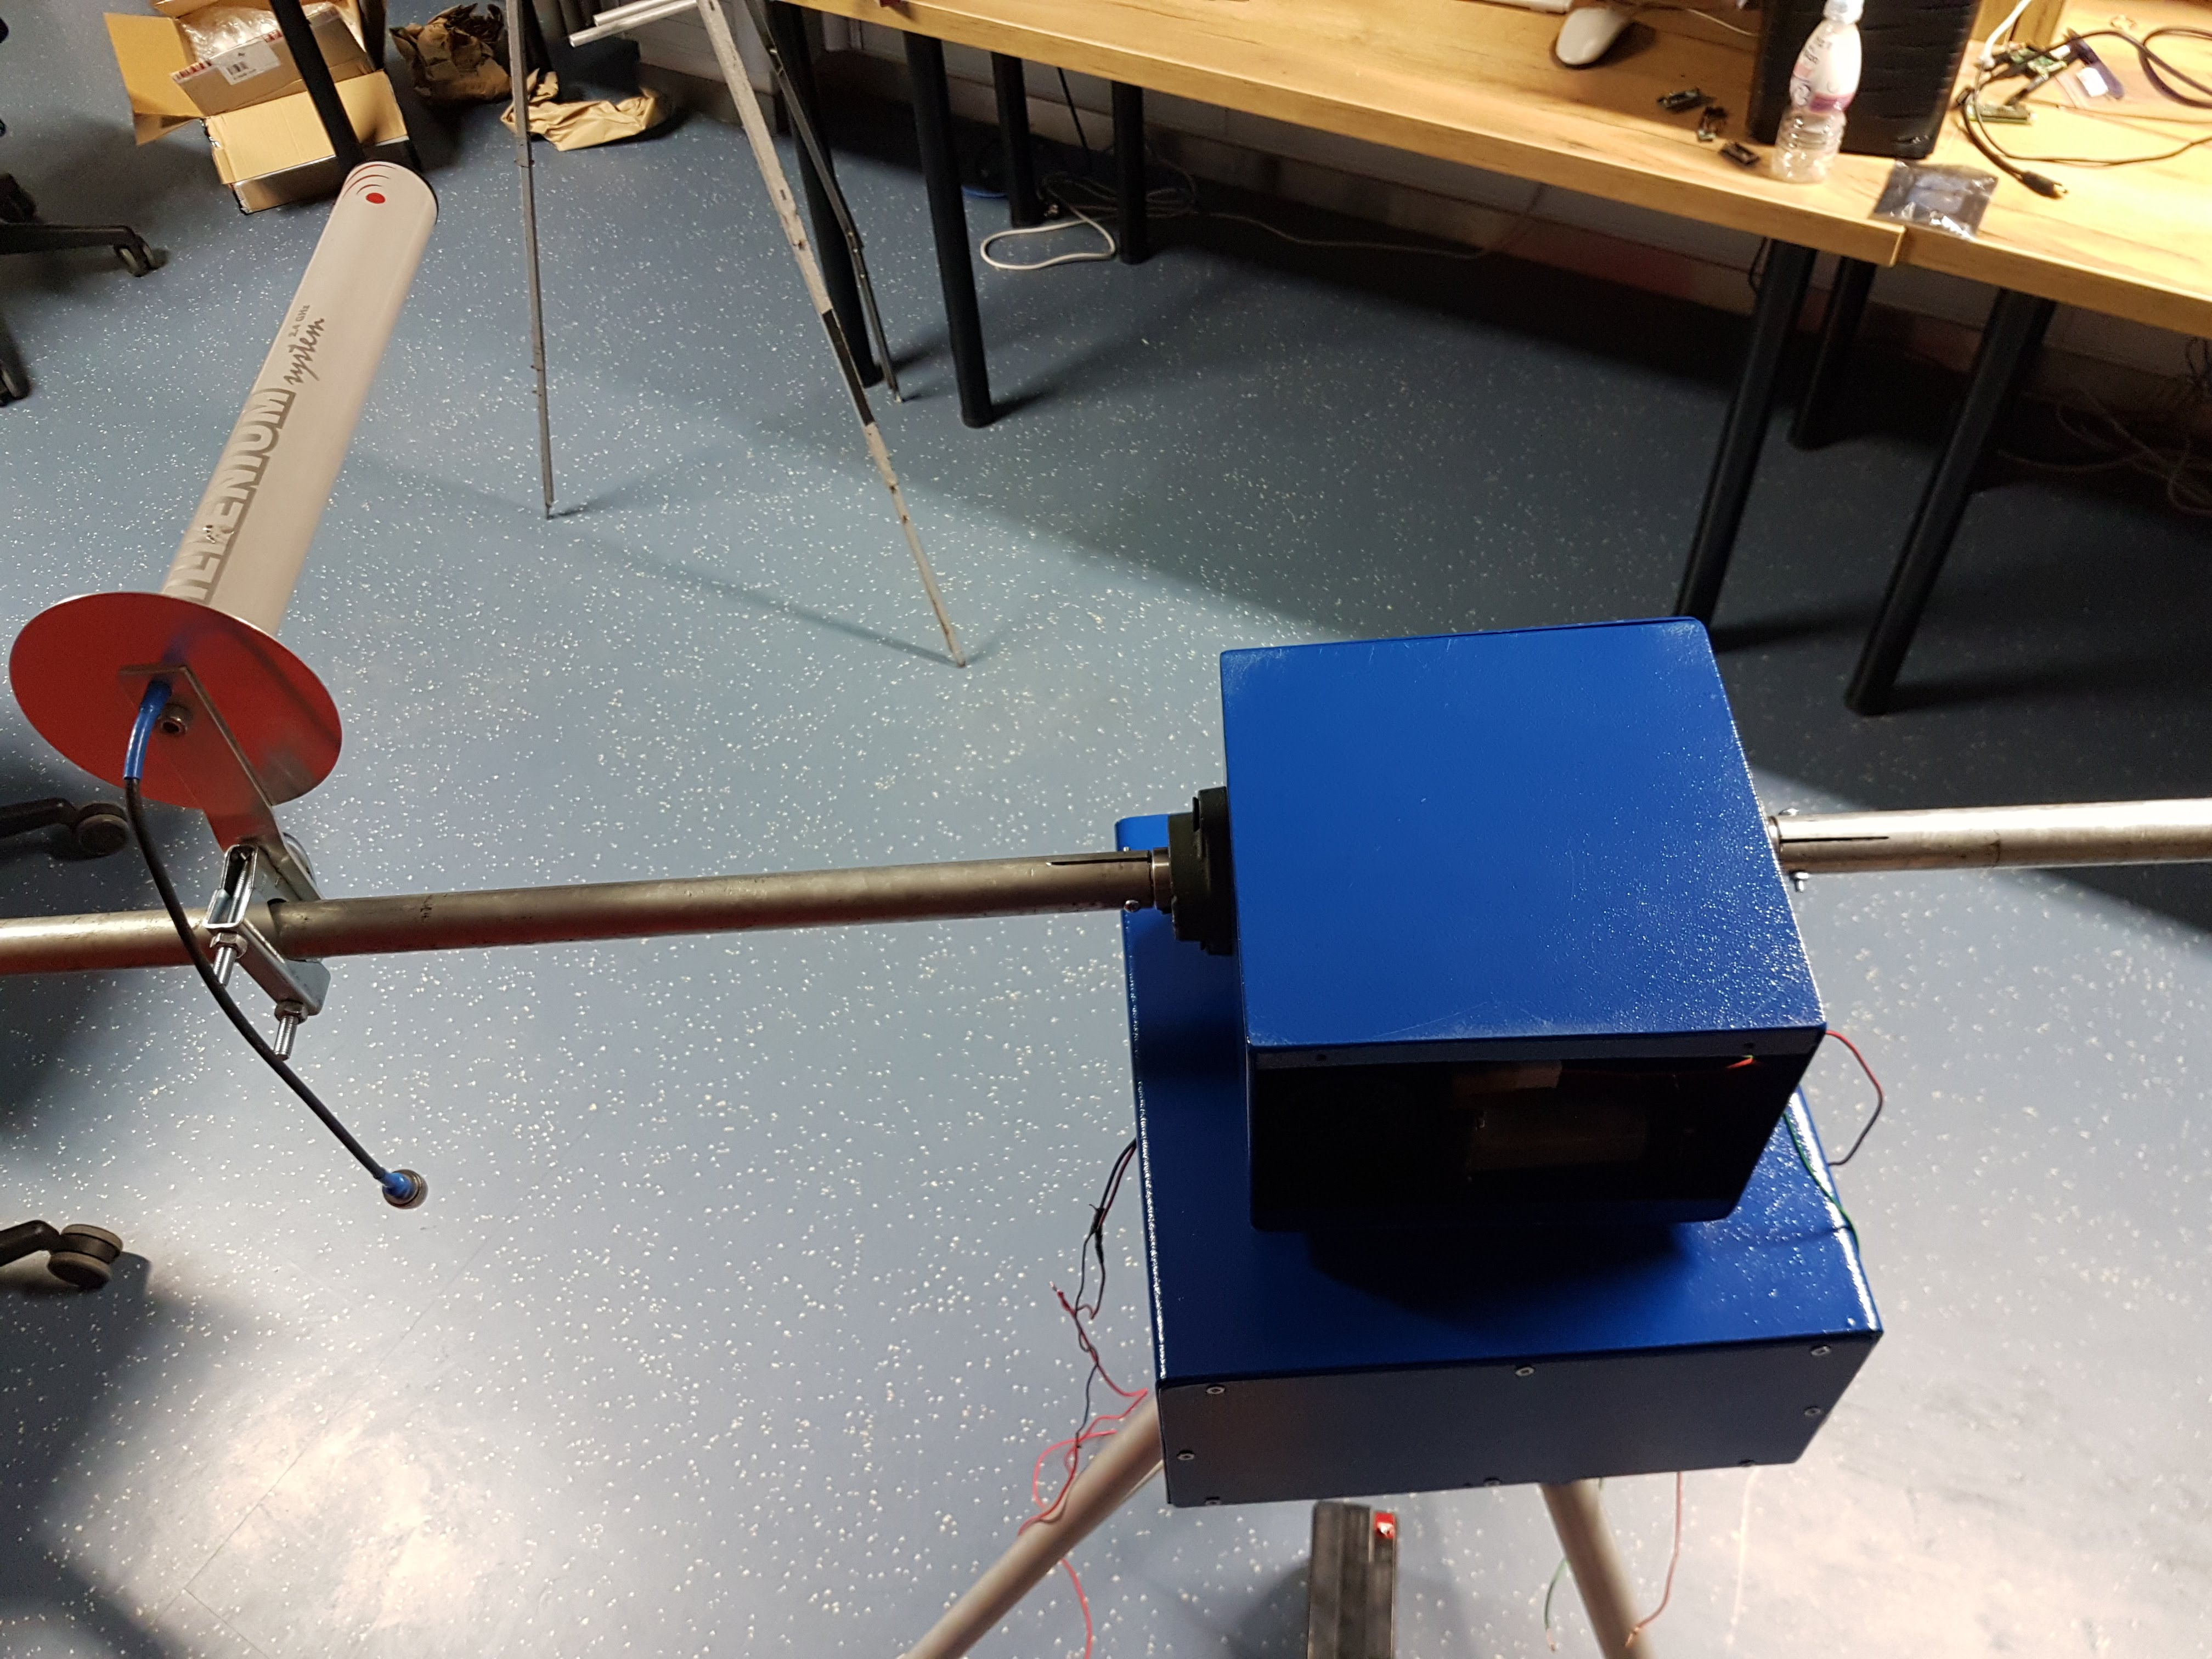
\includegraphics[width=0.7 \textwidth]{testy/antenaS}
	\caption{Antena wskazuje kierunek południowy}	
	\label{fig:antenaS}
\end{figure}

\begin{figure}[h]
	\centering
		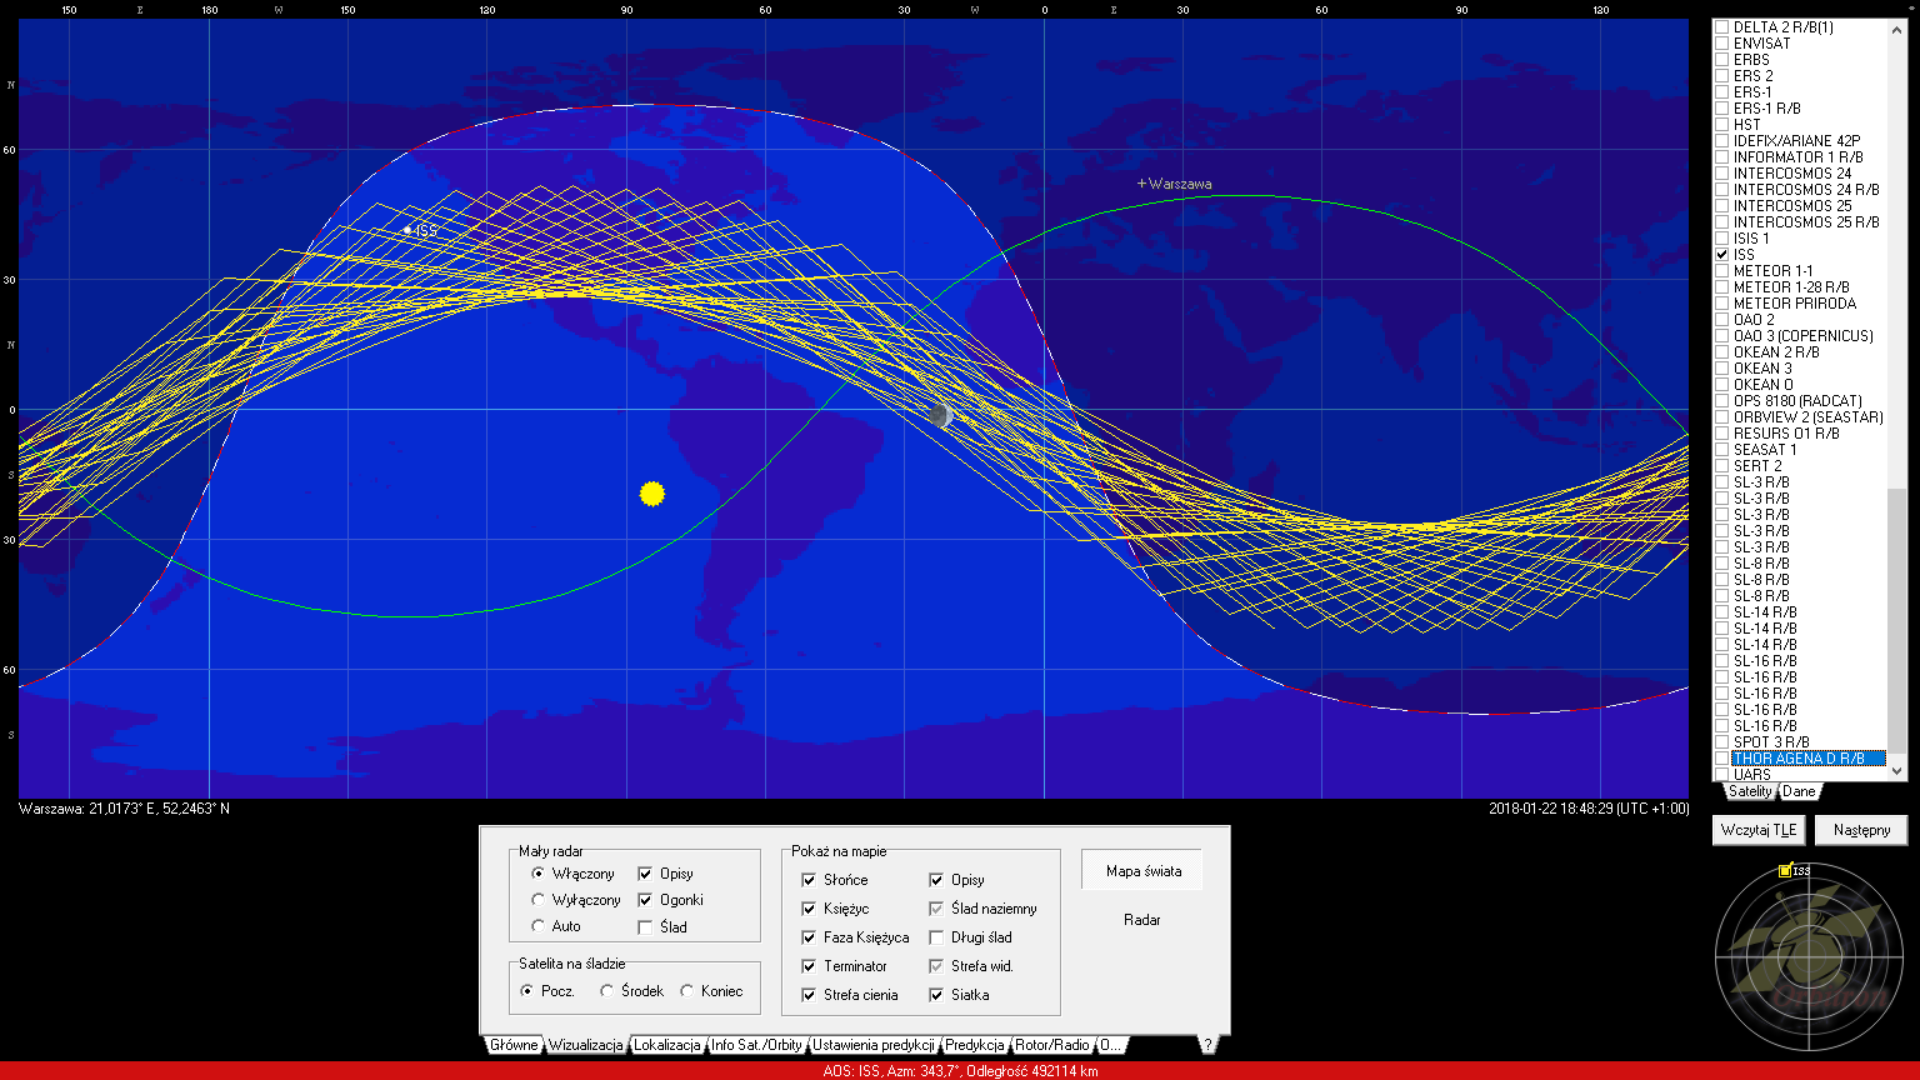
\includegraphics[width=0.7 \textwidth]{testy/pojawia}
	\caption{Satelita ISS pojawia się nad horyzontem}	
	\label{fig:pojawia}
\end{figure}

\begin{figure}[h]
	\centering
		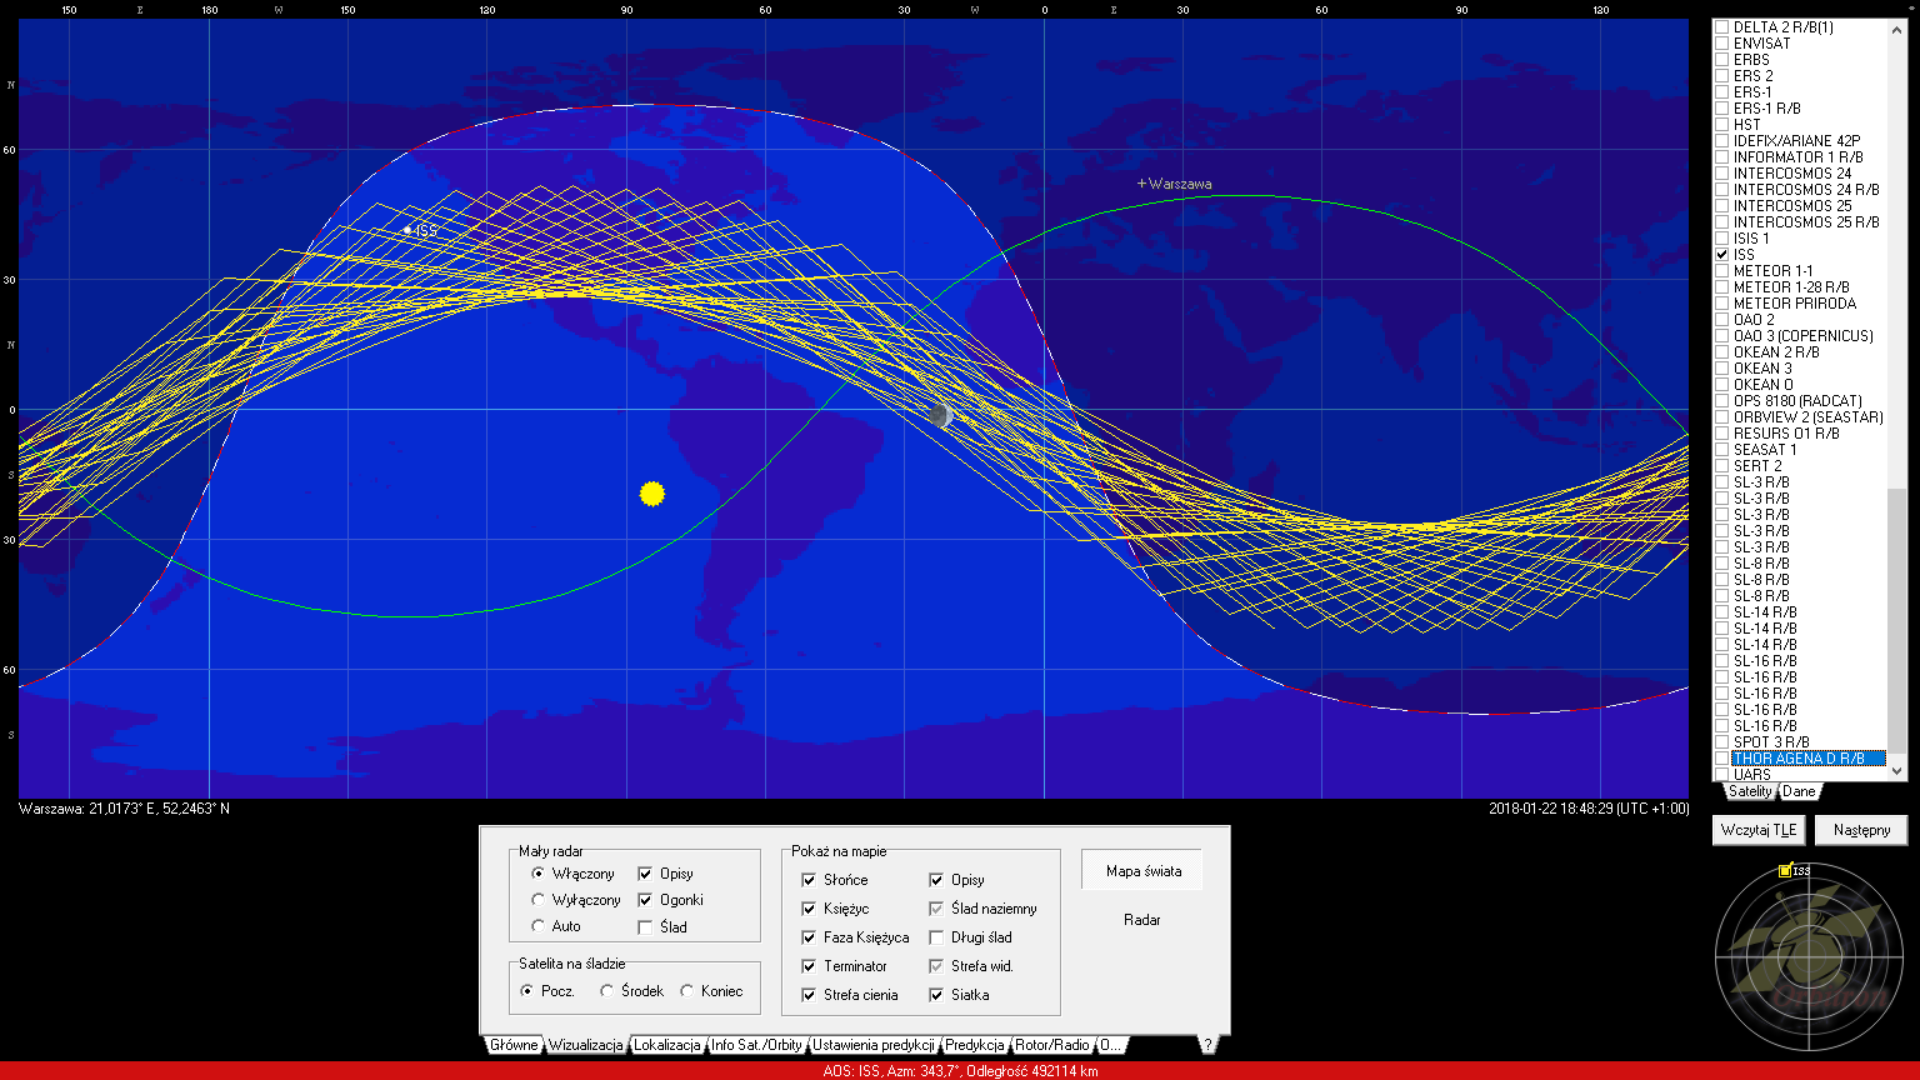
\includegraphics[width=0.7 \textwidth]{testy/pojawia}
	\caption{Satelita ISS pojawia się nad horyzontem}	
	\label{fig:pojawia}
\end{figure}


\begin{figure}[h]
	\centering
		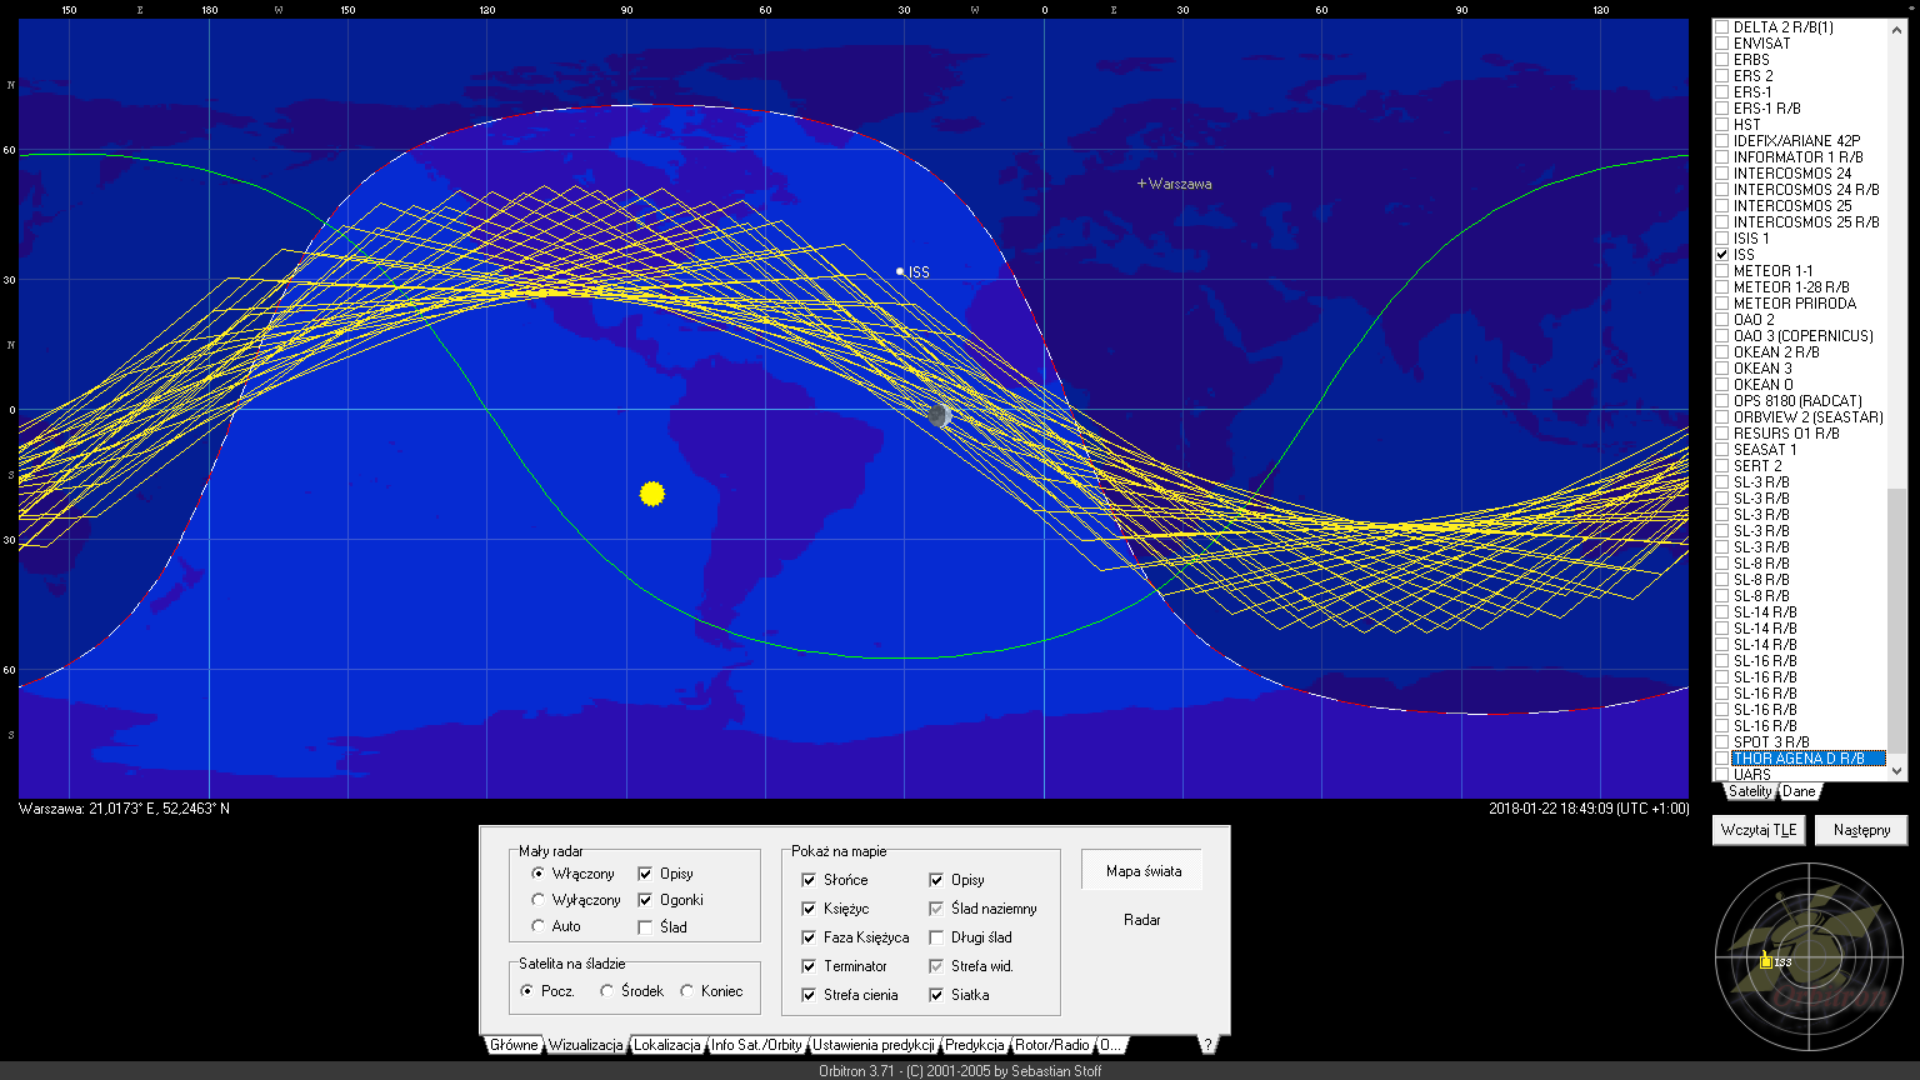
\includegraphics[width=0.7 \textwidth]{testy/zenit}
	\caption{Satelita ISS w zenicie}	
	\label{fig:zenit}
\end{figure}


\begin{figure}[h]
	\centering
		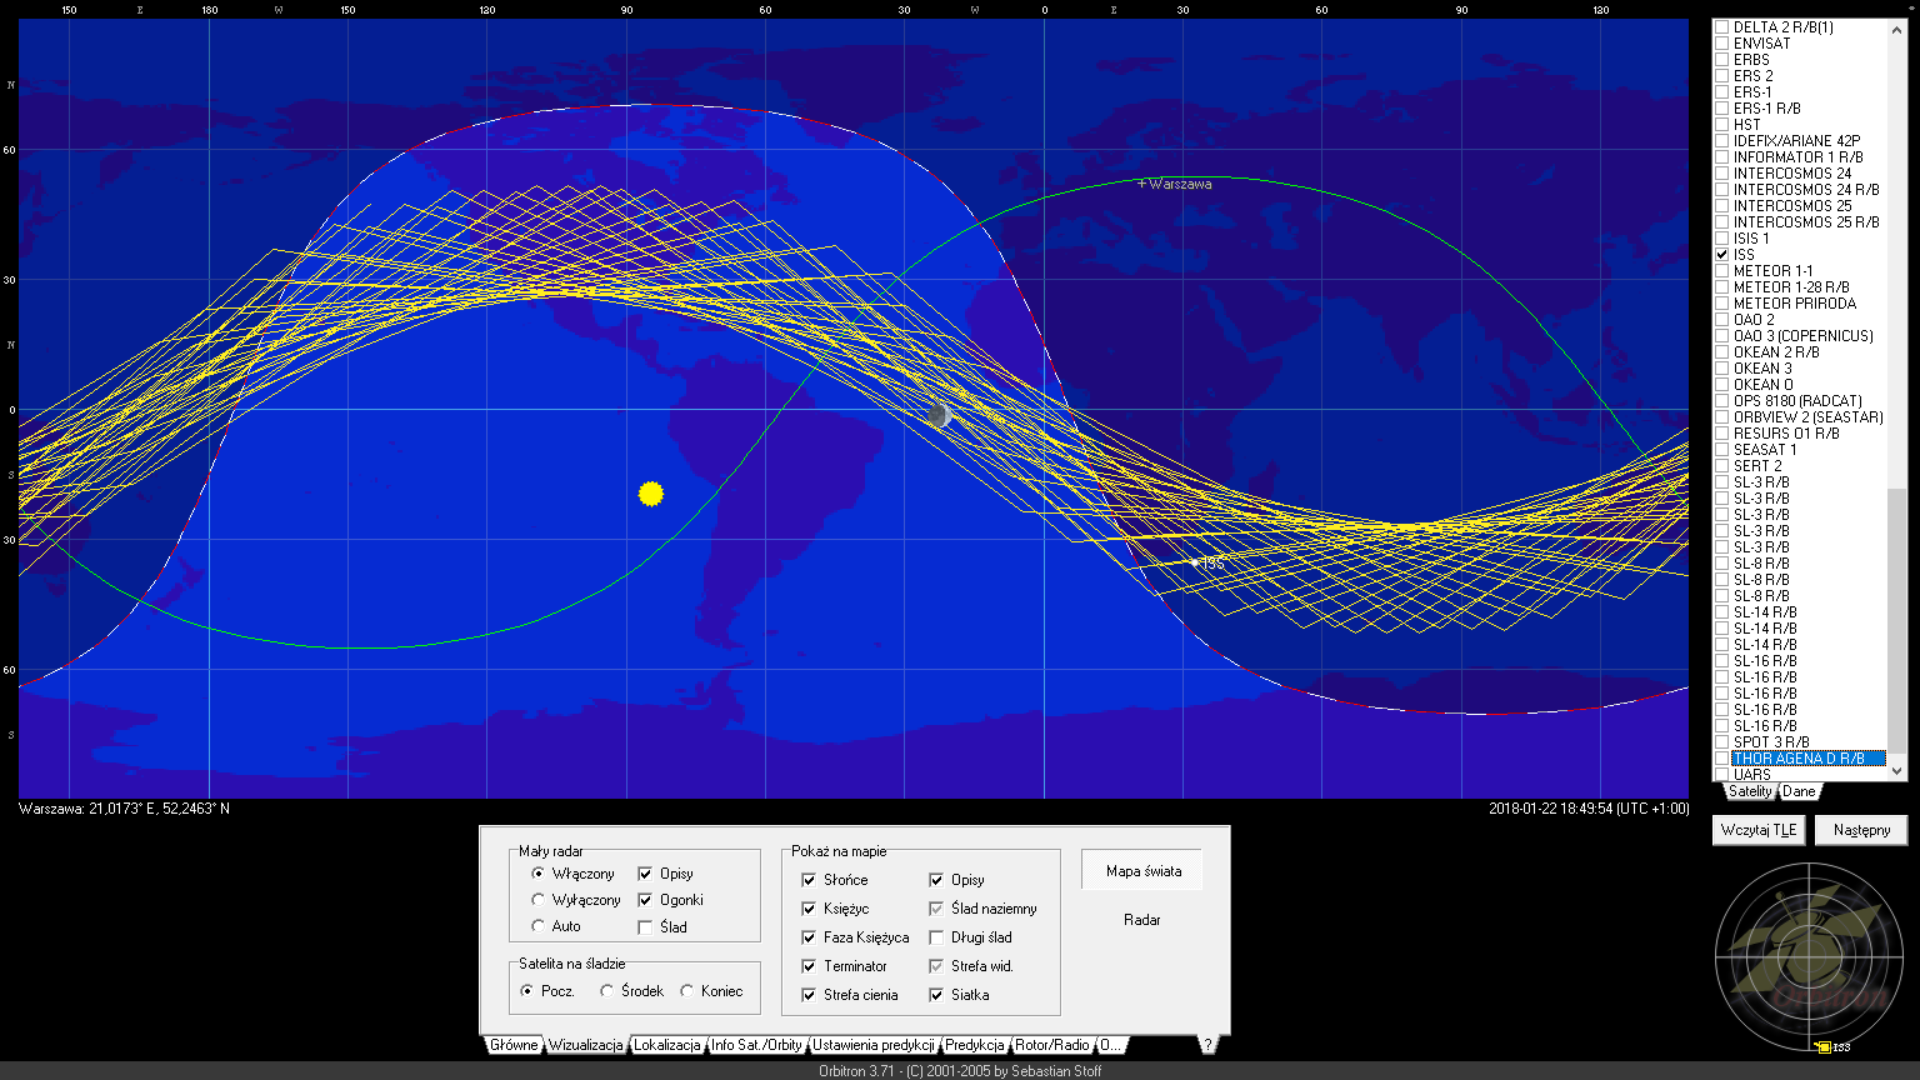
\includegraphics[width=0.7 \textwidth]{testy/znika}
	\caption{Satelita ISS znika za horyzontem}	
	\label{fig:zanika}
\end{figure}




\subsection{Część radiowa}

W części radiowej nie wykonywaliśmy dużo testów. Testowaliśmy jedynie poprawność programu radia programowalnego SDR.

\subsection{Podsumowanie}

Projekt stacji został wykonany pomyślnie. Zaplanowano jeszcze montaż rotora na bagażnik dachowy samochodu, ale nie było to priorytetem. Dokończymy tę realizację przy przygotowaniu misji balonowej, gdzie planowaliśmy śledzić balon jadąc samochodem.
